\documentclass[a4paper]{article}
\usepackage{amsfonts}
\usepackage{amsmath}
\usepackage{amssymb}
\usepackage{graphicx}  
\usepackage{cancel}

\newcommand{\degree}{^{\circ}}
\newcommand{\cis}{\operatorname{cis}}
\newcommand{\Bgsin}{\operatorname{Bgsin}}
\newcommand{\Bgcos}{\operatorname{Bgcos}}
\newcommand{\Bgtan}{\operatorname{Bgtan}}
\newcommand{\limit}{\lim\limits}
\newcommand{\summation}{\displaystyle\sum}
\newcommand{\dom}{\operatorname{dom}}
\newcommand{\Int}{\displaystyle\int}

\begin{document}
  
\noindent \large Auteur: Rune Suy \\
\noindent \large Studierichting: Informatica\\
\noindent \large Oefeningenreeks 5G nr. 6.8\\

\medskip

\normalsize

$f(x)=\sqrt{x}$ en $g(x)=x^2$\\

$x^2 = \sqrt{x} \Leftrightarrow x=x^4 \Leftrightarrow x=0$ of $x=1$\\

$V=\pi \Int_0^1 (\sqrt{x}^2-x^4)dx = \pi\Int_0^1(x-x^4)dx$\\

$= \pi \left[ \left[\dfrac{x^2}{2}\right]_0^1 -  \left[\dfrac{x^5}{5}\right]_0^1\right] = \pi\left( \dfrac{1}{2} - \dfrac{1}{5} \right) = \dfrac{3\pi}{10}$\\

\begin{figure}[h]
\centering
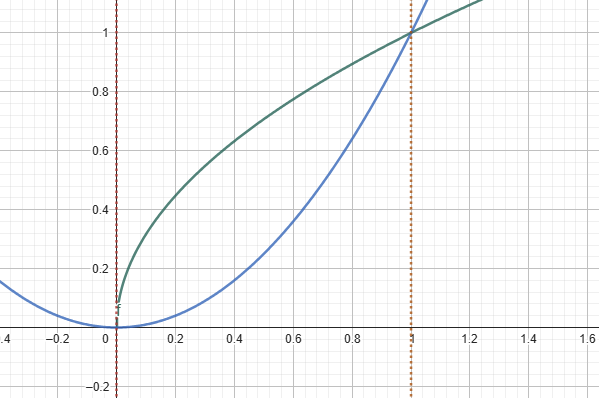
\includegraphics[width=\linewidth]{5G-6.8-rune.suy.INF.png}
\end{figure}

\begin{thebibliography}{999}
%\bibitem{a} Referentie
\end{thebibliography}
\end{document} 
